\documentclass{standalone}
\usepackage{tikz}
\usetikzlibrary{patterns, positioning}


\begin{document}
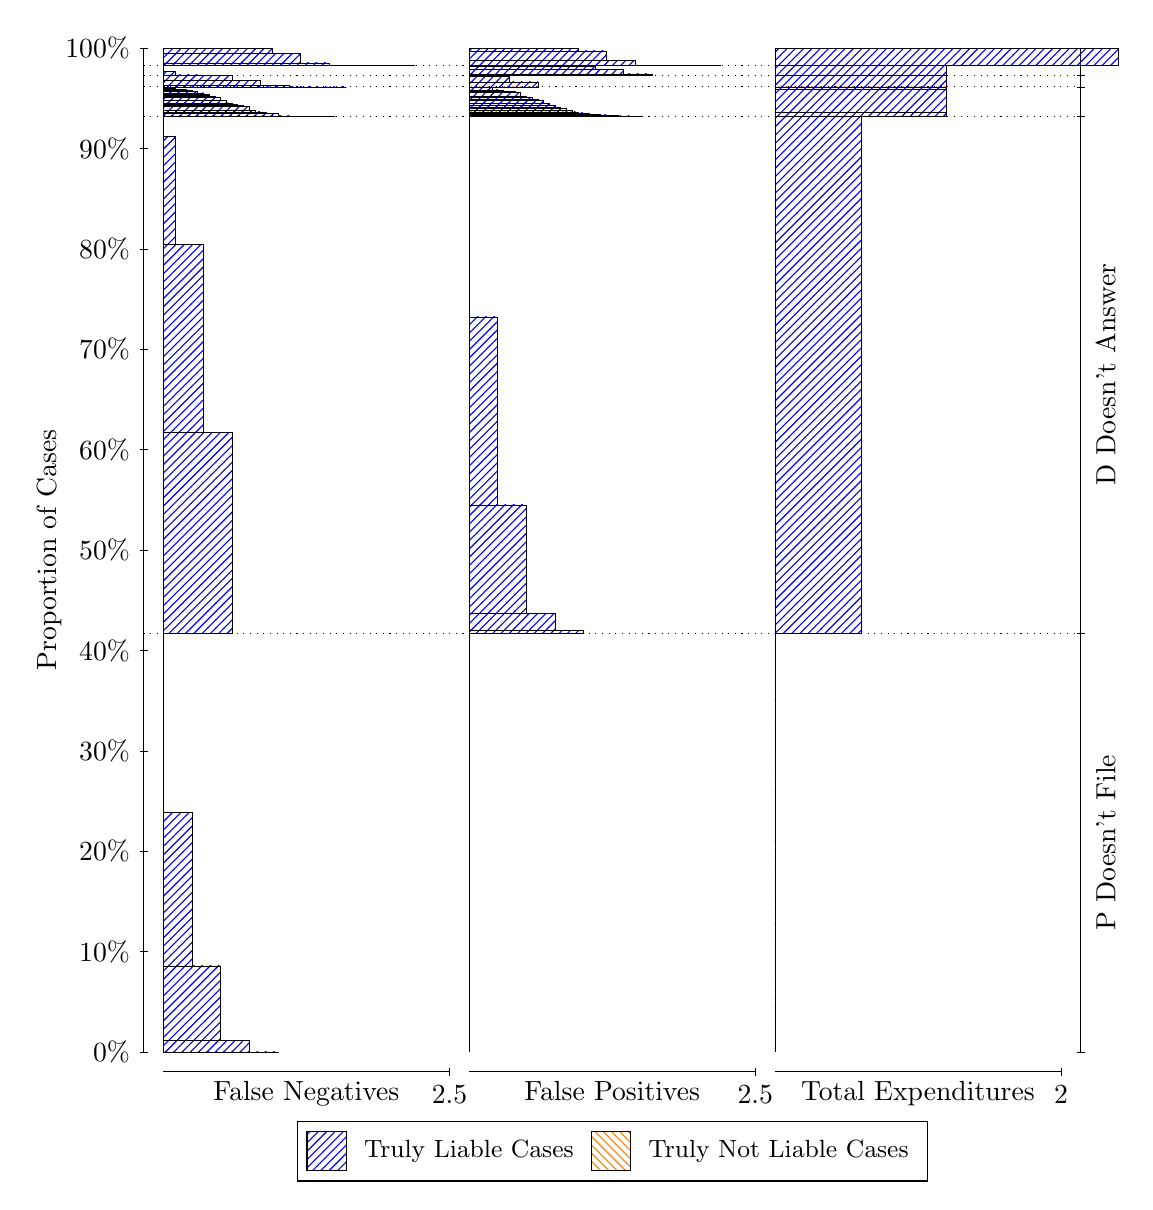
\begin{tikzpicture}
\draw[black, very thin] (1.5,1.75) -- (1.5,14.5);
\node[rotate=90, text=black, anchor=center] at (0.3, 8.125) {Proportion of Cases};
\draw[black, very thin] (1.45,1.75) -- (1.55,1.75);
\node[text=black, anchor=east] at (1.45, 1.75) {0\%};
\draw[black, very thin] (1.45,3.025) -- (1.55,3.025);
\node[text=black, anchor=east] at (1.45, 3.025) {10\%};
\draw[black, very thin] (1.45,4.3) -- (1.55,4.3);
\node[text=black, anchor=east] at (1.45, 4.3) {20\%};
\draw[black, very thin] (1.45,5.575) -- (1.55,5.575);
\node[text=black, anchor=east] at (1.45, 5.575) {30\%};
\draw[black, very thin] (1.45,6.85) -- (1.55,6.85);
\node[text=black, anchor=east] at (1.45, 6.85) {40\%};
\draw[black, very thin] (1.45,8.125) -- (1.55,8.125);
\node[text=black, anchor=east] at (1.45, 8.125) {50\%};
\draw[black, very thin] (1.45,9.4) -- (1.55,9.4);
\node[text=black, anchor=east] at (1.45, 9.4) {60\%};
\draw[black, very thin] (1.45,10.675) -- (1.55,10.675);
\node[text=black, anchor=east] at (1.45, 10.675) {70\%};
\draw[black, very thin] (1.45,11.95) -- (1.55,11.95);
\node[text=black, anchor=east] at (1.45, 11.95) {80\%};
\draw[black, very thin] (1.45,13.225) -- (1.55,13.225);
\node[text=black, anchor=east] at (1.45, 13.225) {90\%};
\draw[black, very thin] (1.45,14.5) -- (1.55,14.5);
\node[text=black, anchor=east] at (1.45, 14.5) {100\%};

\draw[black, very thin] (13.4,1.75) -- (13.4,14.5);
\draw[black, very thin] (13.35,1.75) -- (13.45,1.75);
\node[anchor=west] at (13.35, 1.75) {};
\draw[black, very thin] (13.35,7.0681) -- (13.45,7.0681);
\node[anchor=west] at (13.35, 7.0681) {};
\draw[black, very thin] (13.35,13.634) -- (13.45,13.634);
\node[anchor=west] at (13.35, 13.634) {};
\draw[black, very thin] (13.35,14.006) -- (13.45,14.006);
\node[anchor=west] at (13.35, 14.006) {};
\draw[black, very thin] (13.35,14.155) -- (13.45,14.155);
\node[anchor=west] at (13.35, 14.155) {};
\draw[black, very thin] (13.35,14.276) -- (13.45,14.276);
\node[anchor=west] at (13.35, 14.276) {};
\draw[black, very thin] (13.35,14.5) -- (13.45,14.5);
\node[anchor=west] at (13.35, 14.5) {};

\draw[black, very thin, pattern color=blue, pattern=north east lines] (1.75,1.75) rectangle (3.2033,1.7514);
\draw[black, very thin, pattern color=blue, pattern=north east lines] (1.75,1.7514) rectangle (2.84,1.8956);
\draw[black, very thin, pattern color=blue, pattern=north east lines] (1.75,1.8956) rectangle (2.4767,2.8437);
\draw[black, very thin, pattern color=blue, pattern=north east lines] (1.75,2.8437) rectangle (2.1133,4.7937);
\draw[black, very thin, pattern color=orange, pattern=north west lines] (1.75,4.7937) rectangle (1.75,4.7937);
\draw[black, very thin, pattern color=blue, pattern=north east lines] (1.75,4.7937) rectangle (1.75,7.0681);
\draw[black, very thin, pattern color=blue, pattern=north east lines] (1.75,7.0681) rectangle (2.622,9.6164);
\draw[black, very thin, pattern color=blue, pattern=north east lines] (1.75,9.6164) rectangle (2.2587,12.005);
\draw[black, very thin, pattern color=blue, pattern=north east lines] (1.75,12.005) rectangle (1.8953,13.382);
\draw[black, very thin, pattern color=orange, pattern=north west lines] (1.75,13.382) rectangle (1.75,13.382);
\draw[black, very thin, pattern color=blue, pattern=north east lines] (1.75,13.382) rectangle (1.75,13.634);
\draw[black, very thin, pattern color=blue, pattern=north east lines] (1.75,13.634) rectangle (3.93,13.634);
\draw[black, very thin, pattern color=blue, pattern=north east lines] (1.75,13.634) rectangle (3.7847,13.634);
\draw[black, very thin, pattern color=blue, pattern=north east lines] (1.75,13.634) rectangle (3.6393,13.634);
\draw[black, very thin, pattern color=blue, pattern=north east lines] (1.75,13.634) rectangle (3.5667,13.636);
\draw[black, very thin, pattern color=blue, pattern=north east lines] (1.75,13.636) rectangle (3.494,13.636);
\draw[black, very thin, pattern color=blue, pattern=north east lines] (1.75,13.636) rectangle (3.4213,13.637);
\draw[black, very thin, pattern color=blue, pattern=north east lines] (1.75,13.637) rectangle (3.3487,13.637);
\draw[black, very thin, pattern color=blue, pattern=north east lines] (1.75,13.637) rectangle (3.276,13.638);
\draw[black, very thin, pattern color=blue, pattern=north east lines] (1.75,13.638) rectangle (3.2033,13.673);
\draw[black, very thin, pattern color=blue, pattern=north east lines] (1.75,13.673) rectangle (3.1307,13.674);
\draw[black, very thin, pattern color=blue, pattern=north east lines] (1.75,13.674) rectangle (3.058,13.674);
\draw[black, very thin, pattern color=blue, pattern=north east lines] (1.75,13.674) rectangle (3.058,13.688);
\draw[black, very thin, pattern color=blue, pattern=north east lines] (1.75,13.688) rectangle (2.9853,13.689);
\draw[black, very thin, pattern color=blue, pattern=north east lines] (1.75,13.689) rectangle (2.9127,13.707);
\draw[black, very thin, pattern color=blue, pattern=north east lines] (1.75,13.707) rectangle (2.9127,13.707);
\draw[black, very thin, pattern color=blue, pattern=north east lines] (1.75,13.707) rectangle (2.84,13.756);
\draw[black, very thin, pattern color=blue, pattern=north east lines] (1.75,13.756) rectangle (2.7673,13.767);
\draw[black, very thin, pattern color=blue, pattern=north east lines] (1.75,13.767) rectangle (2.6947,13.769);
\draw[black, very thin, pattern color=blue, pattern=north east lines] (1.75,13.769) rectangle (2.6947,13.788);
\draw[black, very thin, pattern color=blue, pattern=north east lines] (1.75,13.788) rectangle (2.622,13.804);
\draw[black, very thin, pattern color=blue, pattern=north east lines] (1.75,13.804) rectangle (2.5493,13.837);
\draw[black, very thin, pattern color=blue, pattern=north east lines] (1.75,13.837) rectangle (2.5493,13.838);
\draw[black, very thin, pattern color=blue, pattern=north east lines] (1.75,13.838) rectangle (2.4767,13.873);
\draw[black, very thin, pattern color=blue, pattern=north east lines] (1.75,13.873) rectangle (2.404,13.879);
\draw[black, very thin, pattern color=blue, pattern=north east lines] (1.75,13.879) rectangle (2.404,13.888);
\draw[black, very thin, pattern color=blue, pattern=north east lines] (1.75,13.888) rectangle (2.3313,13.896);
\draw[black, very thin, pattern color=blue, pattern=north east lines] (1.75,13.896) rectangle (2.3313,13.909);
\draw[black, very thin, pattern color=blue, pattern=north east lines] (1.75,13.909) rectangle (2.2587,13.929);
\draw[black, very thin, pattern color=blue, pattern=north east lines] (1.75,13.929) rectangle (2.186,13.948);
\draw[black, very thin, pattern color=blue, pattern=north east lines] (1.75,13.948) rectangle (2.186,13.951);
\draw[black, very thin, pattern color=blue, pattern=north east lines] (1.75,13.951) rectangle (2.1133,13.965);
\draw[black, very thin, pattern color=blue, pattern=north east lines] (1.75,13.965) rectangle (2.0407,13.967);
\draw[black, very thin, pattern color=blue, pattern=north east lines] (1.75,13.967) rectangle (2.0407,13.971);
\draw[black, very thin, pattern color=blue, pattern=north east lines] (1.75,13.971) rectangle (1.968,13.981);
\draw[black, very thin, pattern color=blue, pattern=north east lines] (1.75,13.981) rectangle (1.8953,13.987);
\draw[black, very thin, pattern color=blue, pattern=north east lines] (1.75,13.987) rectangle (1.8227,13.991);
\draw[black, very thin, pattern color=orange, pattern=north west lines] (1.75,13.991) rectangle (1.75,13.991);
\draw[black, very thin, pattern color=blue, pattern=north east lines] (1.75,13.991) rectangle (1.75,14.006);
\draw[black, very thin, pattern color=blue, pattern=north east lines] (1.75,14.006) rectangle (4.0753,14.006);
\draw[black, very thin, pattern color=blue, pattern=north east lines] (1.75,14.006) rectangle (3.712,14.007);
\draw[black, very thin, pattern color=blue, pattern=north east lines] (1.75,14.007) rectangle (3.3487,14.026);
\draw[black, very thin, pattern color=blue, pattern=north east lines] (1.75,14.026) rectangle (2.9853,14.09);
\draw[black, very thin, pattern color=blue, pattern=north east lines] (1.75,14.09) rectangle (2.622,14.155);
\draw[black, very thin, pattern color=orange, pattern=north west lines] (1.75,14.155) rectangle (1.75,14.155);
\draw[black, very thin, pattern color=blue, pattern=north east lines] (1.75,14.155) rectangle (2.622,14.155);
\draw[black, very thin, pattern color=blue, pattern=north east lines] (1.75,14.155) rectangle (2.2587,14.16);
\draw[black, very thin, pattern color=blue, pattern=north east lines] (1.75,14.16) rectangle (1.8953,14.202);
\draw[black, very thin, pattern color=orange, pattern=north west lines] (1.75,14.202) rectangle (1.75,14.202);
\draw[black, very thin, pattern color=blue, pattern=north east lines] (1.75,14.202) rectangle (1.75,14.276);
\draw[black, very thin, pattern color=blue, pattern=north east lines] (1.75,14.276) rectangle (4.9473,14.276);
\draw[black, very thin, pattern color=blue, pattern=north east lines] (1.75,14.276) rectangle (4.584,14.276);
\draw[black, very thin, pattern color=blue, pattern=north east lines] (1.75,14.276) rectangle (4.2207,14.277);
\draw[black, very thin, pattern color=blue, pattern=north east lines] (1.75,14.277) rectangle (3.8573,14.311);
\draw[black, very thin, pattern color=blue, pattern=north east lines] (1.75,14.311) rectangle (3.494,14.436);
\draw[black, very thin, pattern color=blue, pattern=north east lines] (1.75,14.436) rectangle (3.1307,14.494);
\draw[black, very thin, pattern color=blue, pattern=north east lines] (1.75,14.494) rectangle (2.7673,14.5);
\draw[black, very thin, pattern color=blue, pattern=north east lines] (1.75,14.5) rectangle (2.404,14.5);
\draw[black, very thin, pattern color=blue, pattern=north east lines] (1.75,14.5) rectangle (2.0407,14.5);
\draw[black, very thin, pattern color=orange, pattern=north west lines] (1.75,14.5) rectangle (1.75,14.5);
\draw[black, very thin, pattern color=orange, pattern=north west lines] (5.6333,1.75) rectangle (5.6333,1.75);
\draw[black, very thin, pattern color=blue, pattern=north east lines] (5.6333,1.75) rectangle (5.6333,7.0681);
\draw[black, very thin, pattern color=orange, pattern=north west lines] (5.6333,7.0681) rectangle (7.0867,7.0681);
\draw[black, very thin, pattern color=blue, pattern=north east lines] (5.6333,7.0681) rectangle (7.0867,7.1029);
\draw[black, very thin, pattern color=blue, pattern=north east lines] (5.6333,7.1029) rectangle (6.7233,7.3197);
\draw[black, very thin, pattern color=blue, pattern=north east lines] (5.6333,7.3197) rectangle (6.36,8.6969);
\draw[black, very thin, pattern color=blue, pattern=north east lines] (5.6333,8.6969) rectangle (5.9967,11.086);
\draw[black, very thin, pattern color=blue, pattern=north east lines] (5.6333,11.086) rectangle (5.6333,13.634);
\draw[black, very thin, pattern color=orange, pattern=north west lines] (5.6333,13.634) rectangle (7.8133,13.634);
\draw[black, very thin, pattern color=blue, pattern=north east lines] (5.6333,13.634) rectangle (7.8133,13.636);
\draw[black, very thin, pattern color=orange, pattern=north west lines] (5.6333,13.636) rectangle (7.668,13.636);
\draw[black, very thin, pattern color=blue, pattern=north east lines] (5.6333,13.636) rectangle (7.668,13.638);
\draw[black, very thin, pattern color=orange, pattern=north west lines] (5.6333,13.638) rectangle (7.5227,13.638);
\draw[black, very thin, pattern color=blue, pattern=north east lines] (5.6333,13.638) rectangle (7.5227,13.641);
\draw[black, very thin, pattern color=blue, pattern=north east lines] (5.6333,13.641) rectangle (7.45,13.645);
\draw[black, very thin, pattern color=orange, pattern=north west lines] (5.6333,13.645) rectangle (7.3773,13.645);
\draw[black, very thin, pattern color=blue, pattern=north east lines] (5.6333,13.645) rectangle (7.3773,13.65);
\draw[black, very thin, pattern color=blue, pattern=north east lines] (5.6333,13.65) rectangle (7.3047,13.653);
\draw[black, very thin, pattern color=orange, pattern=north west lines] (5.6333,13.653) rectangle (7.232,13.653);
\draw[black, very thin, pattern color=blue, pattern=north east lines] (5.6333,13.653) rectangle (7.232,13.66);
\draw[black, very thin, pattern color=blue, pattern=north east lines] (5.6333,13.66) rectangle (7.1593,13.669);
\draw[black, very thin, pattern color=orange, pattern=north west lines] (5.6333,13.669) rectangle (7.0867,13.669);
\draw[black, very thin, pattern color=blue, pattern=north east lines] (5.6333,13.669) rectangle (7.0867,13.675);
\draw[black, very thin, pattern color=blue, pattern=north east lines] (5.6333,13.675) rectangle (7.014,13.689);
\draw[black, very thin, pattern color=orange, pattern=north west lines] (5.6333,13.689) rectangle (6.9413,13.689);
\draw[black, very thin, pattern color=blue, pattern=north east lines] (5.6333,13.689) rectangle (6.9413,13.712);
\draw[black, very thin, pattern color=blue, pattern=north east lines] (5.6333,13.712) rectangle (6.8687,13.732);
\draw[black, very thin, pattern color=orange, pattern=north west lines] (5.6333,13.732) rectangle (6.796,13.732);
\draw[black, very thin, pattern color=blue, pattern=north east lines] (5.6333,13.732) rectangle (6.796,13.745);
\draw[black, very thin, pattern color=blue, pattern=north east lines] (5.6333,13.745) rectangle (6.796,13.752);
\draw[black, very thin, pattern color=blue, pattern=north east lines] (5.6333,13.752) rectangle (6.7233,13.767);
\draw[black, very thin, pattern color=orange, pattern=north west lines] (5.6333,13.767) rectangle (6.6507,13.767);
\draw[black, very thin, pattern color=blue, pattern=north east lines] (5.6333,13.767) rectangle (6.6507,13.802);
\draw[black, very thin, pattern color=blue, pattern=north east lines] (5.6333,13.802) rectangle (6.578,13.836);
\draw[black, very thin, pattern color=blue, pattern=north east lines] (5.6333,13.836) rectangle (6.5053,13.852);
\draw[black, very thin, pattern color=blue, pattern=north east lines] (5.6333,13.852) rectangle (6.4327,13.871);
\draw[black, very thin, pattern color=blue, pattern=north east lines] (5.6333,13.871) rectangle (6.4327,13.873);
\draw[black, very thin, pattern color=blue, pattern=north east lines] (5.6333,13.873) rectangle (6.36,13.885);
\draw[black, very thin, pattern color=blue, pattern=north east lines] (5.6333,13.885) rectangle (6.2873,13.933);
\draw[black, very thin, pattern color=blue, pattern=north east lines] (5.6333,13.933) rectangle (6.2147,13.951);
\draw[black, very thin, pattern color=blue, pattern=north east lines] (5.6333,13.951) rectangle (6.142,13.952);
\draw[black, very thin, pattern color=blue, pattern=north east lines] (5.6333,13.952) rectangle (6.0693,13.966);
\draw[black, very thin, pattern color=blue, pattern=north east lines] (5.6333,13.966) rectangle (6.0693,13.966);
\draw[black, very thin, pattern color=blue, pattern=north east lines] (5.6333,13.966) rectangle (5.9967,13.967);
\draw[black, very thin, pattern color=blue, pattern=north east lines] (5.6333,13.967) rectangle (5.924,14.002);
\draw[black, very thin, pattern color=blue, pattern=north east lines] (5.6333,14.002) rectangle (5.8513,14.003);
\draw[black, very thin, pattern color=blue, pattern=north east lines] (5.6333,14.003) rectangle (5.7787,14.003);
\draw[black, very thin, pattern color=blue, pattern=north east lines] (5.6333,14.003) rectangle (5.706,14.004);
\draw[black, very thin, pattern color=blue, pattern=north east lines] (5.6333,14.004) rectangle (5.6333,14.006);
\draw[black, very thin, pattern color=orange, pattern=north west lines] (5.6333,14.006) rectangle (6.5053,14.006);
\draw[black, very thin, pattern color=blue, pattern=north east lines] (5.6333,14.006) rectangle (6.5053,14.071);
\draw[black, very thin, pattern color=blue, pattern=north east lines] (5.6333,14.071) rectangle (6.142,14.136);
\draw[black, very thin, pattern color=blue, pattern=north east lines] (5.6333,14.136) rectangle (5.7787,14.154);
\draw[black, very thin, pattern color=blue, pattern=north east lines] (5.6333,14.154) rectangle (5.6333,14.155);
\draw[black, very thin, pattern color=orange, pattern=north west lines] (5.6333,14.155) rectangle (7.9587,14.155);
\draw[black, very thin, pattern color=blue, pattern=north east lines] (5.6333,14.155) rectangle (7.9587,14.171);
\draw[black, very thin, pattern color=blue, pattern=north east lines] (5.6333,14.171) rectangle (7.5953,14.228);
\draw[black, very thin, pattern color=blue, pattern=north east lines] (5.6333,14.228) rectangle (7.232,14.271);
\draw[black, very thin, pattern color=blue, pattern=north east lines] (5.6333,14.271) rectangle (6.8687,14.276);
\draw[black, very thin, pattern color=blue, pattern=north east lines] (5.6333,14.276) rectangle (6.5053,14.276);
\draw[black, very thin, pattern color=orange, pattern=north west lines] (5.6333,14.276) rectangle (8.8307,14.276);
\draw[black, very thin, pattern color=blue, pattern=north east lines] (5.6333,14.276) rectangle (8.8307,14.276);
\draw[black, very thin, pattern color=blue, pattern=north east lines] (5.6333,14.276) rectangle (8.4673,14.276);
\draw[black, very thin, pattern color=orange, pattern=north west lines] (5.6333,14.276) rectangle (8.4673,14.276);
\draw[black, very thin, pattern color=blue, pattern=north east lines] (5.6333,14.276) rectangle (8.4673,14.276);
\draw[black, very thin, pattern color=blue, pattern=north east lines] (5.6333,14.276) rectangle (8.104,14.277);
\draw[black, very thin, pattern color=orange, pattern=north west lines] (5.6333,14.277) rectangle (8.104,14.277);
\draw[black, very thin, pattern color=blue, pattern=north east lines] (5.6333,14.277) rectangle (8.104,14.281);
\draw[black, very thin, pattern color=blue, pattern=north east lines] (5.6333,14.281) rectangle (7.7407,14.282);
\draw[black, very thin, pattern color=orange, pattern=north west lines] (5.6333,14.282) rectangle (7.7407,14.282);
\draw[black, very thin, pattern color=blue, pattern=north east lines] (5.6333,14.282) rectangle (7.7407,14.34);
\draw[black, very thin, pattern color=blue, pattern=north east lines] (5.6333,14.34) rectangle (7.3773,14.34);
\draw[black, very thin, pattern color=orange, pattern=north west lines] (5.6333,14.34) rectangle (7.3773,14.34);
\draw[black, very thin, pattern color=blue, pattern=north east lines] (5.6333,14.34) rectangle (7.3773,14.465);
\draw[black, very thin, pattern color=blue, pattern=north east lines] (5.6333,14.465) rectangle (7.014,14.499);
\draw[black, very thin, pattern color=blue, pattern=north east lines] (5.6333,14.499) rectangle (6.6507,14.5);
\draw[black, very thin, pattern color=blue, pattern=north east lines] (5.6333,14.5) rectangle (6.2873,14.5);
\draw[black, very thin, pattern color=blue, pattern=north east lines] (5.6333,14.5) rectangle (5.924,14.5);
\draw[black, very thin, pattern color=orange, pattern=north west lines] (9.5167,1.75) rectangle (9.5167,1.75);
\draw[black, very thin, pattern color=blue, pattern=north east lines] (9.5167,1.75) rectangle (9.5167,7.0681);
\draw[black, very thin, pattern color=orange, pattern=north west lines] (9.5167,7.0681) rectangle (10.607,7.0681);
\draw[black, very thin, pattern color=blue, pattern=north east lines] (9.5167,7.0681) rectangle (10.607,13.634);
\draw[black, very thin, pattern color=orange, pattern=north west lines] (9.5167,13.634) rectangle (11.697,13.634);
\draw[black, very thin, pattern color=blue, pattern=north east lines] (9.5167,13.634) rectangle (11.697,13.678);
\draw[black, very thin, pattern color=orange, pattern=north west lines] (9.5167,13.678) rectangle (11.697,13.678);
\draw[black, very thin, pattern color=blue, pattern=north east lines] (9.5167,13.678) rectangle (11.697,13.974);
\draw[black, very thin, pattern color=orange, pattern=north west lines] (9.5167,13.974) rectangle (11.697,13.974);
\draw[black, very thin, pattern color=blue, pattern=north east lines] (9.5167,13.974) rectangle (11.697,14.006);
\draw[black, very thin, pattern color=orange, pattern=north west lines] (9.5167,14.006) rectangle (11.697,14.006);
\draw[black, very thin, pattern color=blue, pattern=north east lines] (9.5167,14.006) rectangle (11.697,14.155);
\draw[black, very thin, pattern color=orange, pattern=north west lines] (9.5167,14.155) rectangle (11.697,14.155);
\draw[black, very thin, pattern color=blue, pattern=north east lines] (9.5167,14.155) rectangle (11.697,14.276);
\draw[black, very thin, pattern color=orange, pattern=north west lines] (9.5167,14.276) rectangle (13.877,14.276);
\draw[black, very thin, pattern color=blue, pattern=north east lines] (9.5167,14.276) rectangle (13.877,14.277);
\draw[black, very thin, pattern color=orange, pattern=north west lines] (9.5167,14.277) rectangle (13.877,14.277);
\draw[black, very thin, pattern color=blue, pattern=north east lines] (9.5167,14.277) rectangle (13.877,14.5);
\draw[black, dotted] (1.5,7.0681) -- (13.4,7.0681);
\draw[black, dotted] (1.5,13.634) -- (13.4,13.634);
\draw[black, dotted] (1.5,14.006) -- (13.4,14.006);
\draw[black, dotted] (1.5,14.155) -- (13.4,14.155);
\draw[black, dotted] (1.5,14.276) -- (13.4,14.276);
\draw[black, very thin] (1.75,1.5) -- (5.3833,1.5);
\node[text=black, anchor=north] at (3.5667, 1.5) {False Negatives};
\draw[black, very thin] (5.3833,1.45) -- (5.3833,1.55);
\node[text=black, anchor=north] at (5.3833, 1.45) {2.5};

\draw[black, very thin] (5.6333,1.5) -- (9.2667,1.5);
\node[text=black, anchor=north] at (7.45, 1.5) {False Positives};
\draw[black, very thin] (9.2667,1.45) -- (9.2667,1.55);
\node[text=black, anchor=north] at (9.2667, 1.45) {2.5};

\draw[black, very thin] (9.5167,1.5) -- (13.15,1.5);
\node[text=black, anchor=north] at (11.333, 1.5) {Total Expenditures};
\draw[black, very thin] (13.15,1.45) -- (13.15,1.55);
\node[text=black, anchor=north] at (13.15, 1.45) {2};

\node[text=black, centered, rotate=90] at (13.72, 4.409) {P Doesn't File};
\node[text=black, centered, rotate=90] at (13.72, 10.351) {D Doesn't Answer};





\draw (7.449999999999999,1.5) node[draw=none] (baseCoordinate) {};
\begin{scope}[align=center]
        \matrix[scale=0.5, draw=black, below=0.5cm of baseCoordinate, nodes={draw}, column sep=0.1cm]{
            \node[rectangle, draw, minimum width=0.5cm, minimum height=0.5cm, pattern color=blue, pattern=north east lines] {}; &
            \node[draw=none, font=\small, text=black] (B) {Truly Liable Cases}; &
            \node[rectangle, draw, minimum width=0.5cm, minimum height=0.5cm, pattern color=orange, pattern=north west lines] {}; &
            \node[draw=none, font=\small, text=black] (B) {Truly Not Liable Cases}; \\
            };
\end{scope}

\end{tikzpicture}
\end{document}